\section{Plano de Trabalho e Cronograma de Execução}

O cronograma de execução para essas tarefas ao longo do Doutorado pode ser encontrado na Figura \ref{fig:cronograma}.
As tarefas para essa proposta estão expostas a seguir.

\begin{figure}[ht]
    \centering
    \caption{Cronograma de execução. Siglas: E - estudo aprofundado; D - desenvolvimento de modelo; C - desenvolvimendo (\emph{development}) de código; S - simulação; M - disciplinas; T - dissertação.}
    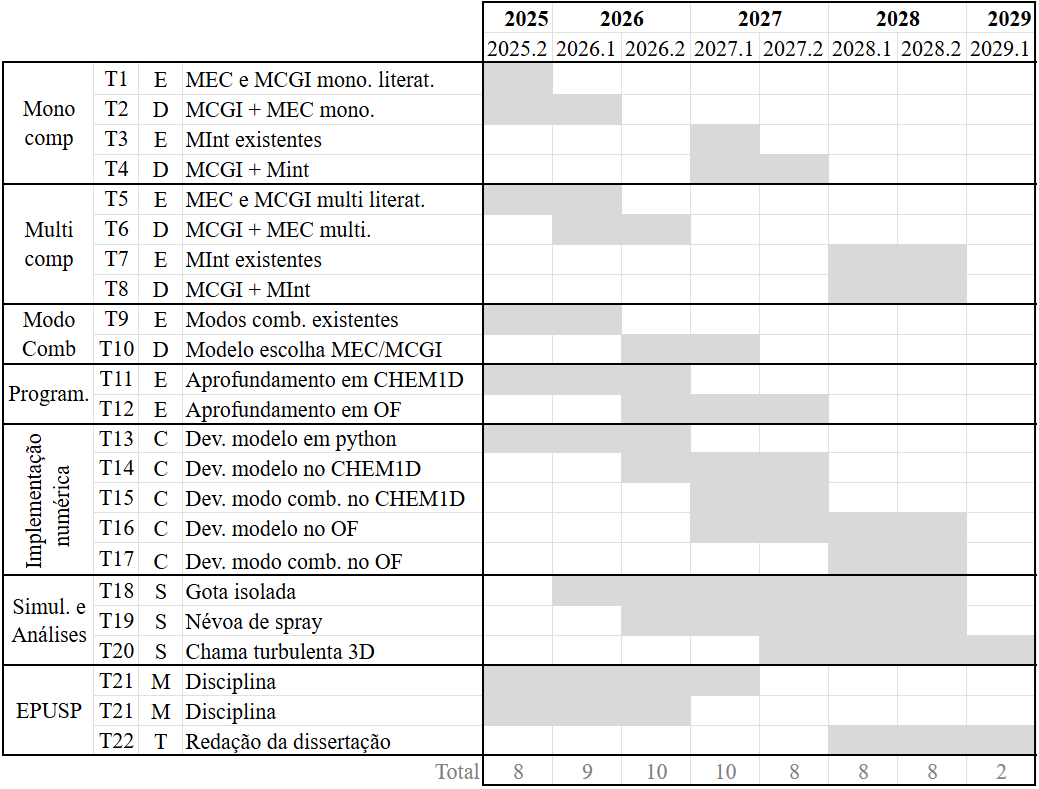
\includegraphics[width=0.9\textwidth]{30_images/cronograma-3.png}
    \label{fig:cronograma}
\end{figure}


Considerando inicialmente gotas monocomponentes, o trabalho proposto se iniciará com o estudo aprofundado sobre MEC e MCGI monocomponentes pré-existentes na literatura (tarefa \textbf{T1}), o que dará base para o desenvolvimento de modelo integral de combustão de gota isolada monocomponente com modelo detalhado de evaporação (tarefa \textbf{T2}).
Em sequência virá o estudo aprofundado de modelos preexistentes para a modelagem de \yellow{de fenômenos de} \yellow{transporte no interior de gota} (tarefa \textbf{T3}), seguido pela avaliação da viabilidade de acoplamento de modelos monocomponente de combustão de gota isolada com discretização no interior da gota (tarefa \textbf{T4}).
A mesma sequência de tarefas procede para gotas multicomponentes, originando respectivamente as tarefas (\textbf{T5}), (\textbf{T6}), (\textbf{T7}) e (\textbf{T8}). 

Visando utilizar o MCGI desenvolvido em simulações de combustão de spray, faz-se necessário então o estudo aprofundado de modelos de modo de combustão de sprays (\textbf{T9}), focando no modo de combustão de gota isolada e de combustão externa. Em seguida propõe-se o desenvolvimento de um modelo para determinar se a gota utiliza um MEC ou MCGI, baseado nos modelos preexistentes na literatura. (\textbf{T10}).

Para simular os modelos desenvolvidos, é necessário implementá-los no programa a ser utilizado.
Assim, torna-se fundamental o estudo aprofundado dos softwares e das linguagens de programação empregadas. 
No caso da simulação em ambiente simplificado, isso envolve o software CHEM1D e a linguagem Fortran (\textbf{T11}).
Já para a simulação turbulenta multidimensional, envolve o software OpenFOAM e a linguagem C++ (\textbf{T12}).
% Em ambos os casos, o aprofundamento na linguagem de programação visa a implementação do modelo desenvolvido no software utilizado.

Dessa forma, as próximas tarefas abordam a implementação dos MEC e MCGIs desenvolvidos: na linguagem Python  (\textbf{T13}), no  CHEM1D à  (\textbf{T14}) e no OpenFOAM  (\textbf{T16}).
Nos dois últimos, é necessário também implementar o algorítimo de seleção entre MEC e MCGI, originando (\textbf{T15}) e (\textbf{T17}).  
% As tarefas (\textbf{T15}) e (\textbf{T17}) referem-se à implementação do algorítmo do modelo de modo de combustão, que fará a escolha entre MEC e MCGI, nos softwares CHEM1D e OpenFOAM respectivamente.

As primeiras simulações dos modelos desenvolvidos são simulações 0D de evolução temporal de gota isolada em Python (\textbf{T18}). 
Em seguida, vêm as simulações de chama combustão laminar em névoa quiescente de spray no CHEM1D (\textbf{T19}).
Por fim, após aprofundamento em interação chama-turbulência, virão as simulações de chama multidimensional turbulenta no OpenFOAM nas grandes escalas, usando LES, FGM, ATG, e os modelos novos (\textbf{T20}).
As tarefas de simulação detalhadas aqui incluem o pré-processamento, o tempo de simulação e a análise dos resultados (pós-processamento).
As ferramentas utilizadas para a análise dos resultados em cada uma das atividades de simulação são discutidas na Seção \ref{sec:resultados}.

O Programa de Pós-Graduação em Engenharia Mecânica (PPGEM) da EPUSP exige que 9 disciplinas sejam cursadas para doutorado direto.
Elas são representadas pela tarefa (\textbf{T21}).
Algumas disciplinas se destacam devido a sua conexão direta com o tema deste projeto: Fundamentos de Combustão I (PME5228), Fundamentos de Escoamentos Turbulentos Reativos (PME5411), Sistemas Particulados (PQI5848), Termodinâmica Avançada I (PME5014), Introdução à Mecânica dos Meios Contínuos (PME5011) e Modelagem de Turbulência para CFD (PME5418).
Demais disciplinas serão definidas ao longo do desenvolvimento deste trabalho.
Por fim, a redação da dissertação é representada pela tarefa (\textbf{T22}).



% \begin{itemize}
% \setlength{\itemsep}{0cm}
% \item[\textbf{T1}] Estudo aprofundado sobre MEC e MCGI monocomponentes pré-existentes na literatura.% Sobre o MEC, estão incluidos o estudo da derivação dos modelos de Abramzon-Sirignano \cite{Sirignano1989}, a formulação de Miller \cite{MillerR1998}, \todo{...}, No que tange a MCGIs, revisitar o modelo de Godsave-Spalding \cite{Law1978,HenningsJ2024MT}, estudar o artigo do Fachini \cite{FachiniF1999}, suas referências e citações, \todo{...} 
% \item[\textbf{T2}] Modelagem analítica de combustão de gota isolada monocomponente com modelo detalhado de evaporação. % Essa tarefa baseia-se na incorporação do modelo de Abramzon-Sirignano \cite{Sirignano1989} ou da formulação de Miller \cite{MillerR1998} no modelo de Godsave-Spalding \cite{Law1978}. %Como todos os modelos citados baseiam-se em soluções analíticas, é visto como provável que 
% \item[\textbf{T3}] Estudo de modelos preexistentes para a modelagem  analítica de discretização do interior de gota monocomponente.% São exemplos de literatura relevante para essa tarefa \source{}.
% \item[\textbf{T4}] Avaliação da viabilidade de acoplamento de modelos monocomponente de combustão de gota isolada com discretização no interior da gota.% Como os modelos de discretização de interior de gota podem envolver soluções numéricas, se será possível desenvolver uma solução analítica para esse problema. Uma solução acoplada numérica-analítica, interna e externamente gota, respectivamente, precisa ser robusta e computacionalmente eficiente para servir em aplicações CFD. 

% \item[\textbf{T5}] Estudo de modelos MEC e MCGI multicomponente preexistentes na literatura.% Exemplos de trabalhos relevantes de MEC multicomponente incluem \source{}.
% \item[\textbf{T6}] Modelagem analítica de combustão de gota isolada multicomponente com modelo avançado de evaporação. % Essa tarefa baseia-se na incorporação dos modelos de Sacomano \cite{SacomanoF2022IJHMT} ou de Wang \source{WangC2012} no modelo de Godsave-Spalding \cite{Law1978}.
% \item[\textbf{T7}] Estudo de modelos preexistentes para a modelagem analítica de discretização do interior de gota multicomponente.% São exemplos de literatura relevante para essa tarefa \source{}
% \item[\textbf{T8}] Avaliação da viabilidade de acoplamento de modelos multicomponente de combustão de gota isolada com discretização no interior da gota. 

% \item[\textbf{T9}] Estudo de modelos de determinação de modos de combustão de gotas de spray, focando no modo de combustão isolada.% São exemplos de literatura relevante para essa tarefa \cite{AggarwalS2014}, \source{}
% \item[\textbf{T10}] Desenvolvimento de modelo analítico para escolha entre MEC e MCGI, baseado na pesquisa do item anterior.

% \item[\textbf{T11}] Aprofundamento em CHEM1D e em Fortran para programação no CHEM1D.
% \item[\textbf{T12}] Aprofundamento em OpenFOAM e em C++ para programação no OpenFOAM.

% \item[\textbf{T13}] Implementação do modelo MEC/MCGI em Python.% para o T18.
% \item[\textbf{T14}] Implementação do modelo MEC/MCGI no CHEM1D.% para o T19.
% \item[\textbf{T15}] Implementação do modelo de modo de combustão no CHEM1D.
% \item[\textbf{T16}] Implementação do modelo MEC/MCGI no OpenFOAM.% para o T20.
% \item[\textbf{T17}] Implementação do modelo de modo de combustão no OF.

% \item[\textbf{T18}] Simulação da evolução temporal 0D de gota isolada em Python.           %, após T15.
% \item[\textbf{T19}] Simulação de combustão laminar de névoa quiescente de spray no CHEM1D. %, após T16.
% \item[\textbf{T20}] Simulação de chama turbulenta 3D nas grandes escalas com FGM e ATF.    %, após T17.

% \item[\textbf{T21}] Disciplinas de pós-graduação.% No programa de Doutorado Direto do PPGEM na POLI-USP, é necessário cursar 9 Disciplinas, cada valendo 8 créditos. Como não é recomendado cursar mais de duas disciplinas por oferencimento, o qual é quadrimestral, as disciplinas serão cursadas ao longo de 5 quadrimestres, aproximadamente 2 anos. Algumas das disciplinas a serem cursadas já foram escolhidas e estão dispostas na Seção \ref{sec:disciplinas}.
% \item[\textbf{T22}] Redação da dissertação.% Estimou-se iniciar a escrita da dissertação nos últimos três semestres.
% \end{itemize}

